\documentclass[12pt,a4paper]{article}
\usepackage[utf8]{inputenc}
\usepackage[T1]{fontenc}
\usepackage{amsmath}
\usepackage{amsfonts}
\usepackage{amssymb}
\usepackage{graphicx}
\usepackage{hyperref}
\usepackage{listings}
\usepackage{xcolor}
\usepackage{booktabs}
\usepackage{float}
\usepackage{enumitem}
\usepackage[left=2.5cm,right=2.5cm,top=2.5cm,bottom=2.5cm]{geometry}

\hypersetup{
    colorlinks=true,
    linkcolor=blue,
    filecolor=magenta,
    urlcolor=cyan,
}

\definecolor{codegreen}{rgb}{0,0.6,0}
\definecolor{codegray}{rgb}{0.5,0.5,0.5}
\definecolor{codepurple}{rgb}{0.58,0,0.82}
\definecolor{backcolour}{rgb}{0.95,0.95,0.95}

\lstdefinestyle{mystyle}{
    backgroundcolor=\color{backcolour},
    commentstyle=\color{codegreen},
    keywordstyle=\color{magenta},
    numberstyle=\tiny\color{codegray},
    stringstyle=\color{codepurple},
    basicstyle=\ttfamily\footnotesize,
    breakatwhitespace=false,
    breaklines=true,
    captionpos=b,
    keepspaces=true,
    numbers=left,
    numbersep=5pt,
    showspaces=false,
    showstringspaces=false,
    showtabs=false,
    tabsize=2
}

\lstset{style=mystyle}
\title{\textbf{keystoneDB}}
\author{
    Group Name: ChadGPT \\
    Mayash Nayak 22CS30064 \\
    Sumit Kumar 22CS30056 \\
    Aviral Singh 22CS300015 \\
    \vspace{1cm}
}
\date{\today}

\begin{document}
\maketitle


\vspace{0.5cm}
\begin{center}
\textbf{Project Link:} keystoneDB: \url{https://github.com/SumitKumar-17/keystoneDB}
\end{center}

\pagebreak

\tableofcontents
\clearpage  % Force content to start on a new page

\section{Introduction}
\subsection{Project Overview}
keystoneDB is an educational DBMS implementation designed to provide hands-on experience with database internals. The system implements a subset of SQL functionality with a focus on understanding the core components of a database management system. The project demonstrates practical implementation of concepts including:

\begin{itemize}
    \item SQL lexical analysis and parsing
    \item Translation of SQL statements to an intermediate representation
    \item Execution of queries using a custom engine
    \item Persistent storage using a key-value store (RocksDB)
    \item Data type implementation and constraint enforcement
    \item Expression evaluation using the visitor pattern
\end{itemize}

\subsection{Educational Goals}
The primary objective of keystoneDB is educational, focusing on:
\begin{itemize}
    \item Understanding compiler design principles in the context of SQL
    \item Gaining practical experience with expression evaluation using the visitor pattern
    \item Learning integration techniques for third-party libraries
    \item Practicing unit testing with GoogleTest
    \item Applying modern C++ programming practices
\end{itemize}

\section{System Architecture}
\subsection{High-Level Architecture}
The keystoneDB system follows a layered architecture typical of database management systems:

\begin{figure}[H]
\centering
\begin{tabular}{|c|}
\hline
\textbf{Client Interface} \\
\hline
\textbf{SQL Parser (Flex/Bison)} \\
\hline
\textbf{Abstract Syntax Tree (AST)} \\
\hline
\textbf{Query Execution Engine} \\
\hline
\textbf{Storage Engine (RocksDB)} \\
\hline
\end{tabular}
\caption{High-level architecture of keystoneDB}
\end{figure}

Each layer has a specific responsibility:
\begin{itemize}
    \item \textbf{Client Interface}: Provides a command-line interface with history and line-editing capabilities
    \item \textbf{SQL Parser}: Converts SQL text into tokens and builds an abstract syntax tree
    \item \textbf{Abstract Syntax Tree}: Represents the structure of SQL statements
    \item \textbf{Query Execution Engine}: Executes the statements represented by the AST
    \item \textbf{Storage Engine}: Handles persistent storage using RocksDB
\end{itemize}

\subsection{Visual Architecture Overview}
keystoneDB's architecture can be visualized through the following component diagrams that illustrate the system's key modules and their interactions.

\clearpage % Force a new page to start the architecture diagrams
\addcontentsline{toc}{subsection}{Architecture Diagrams}

% Pair 1: Component interaction and Parser pipeline
\begin{figure}[h!]
\centering
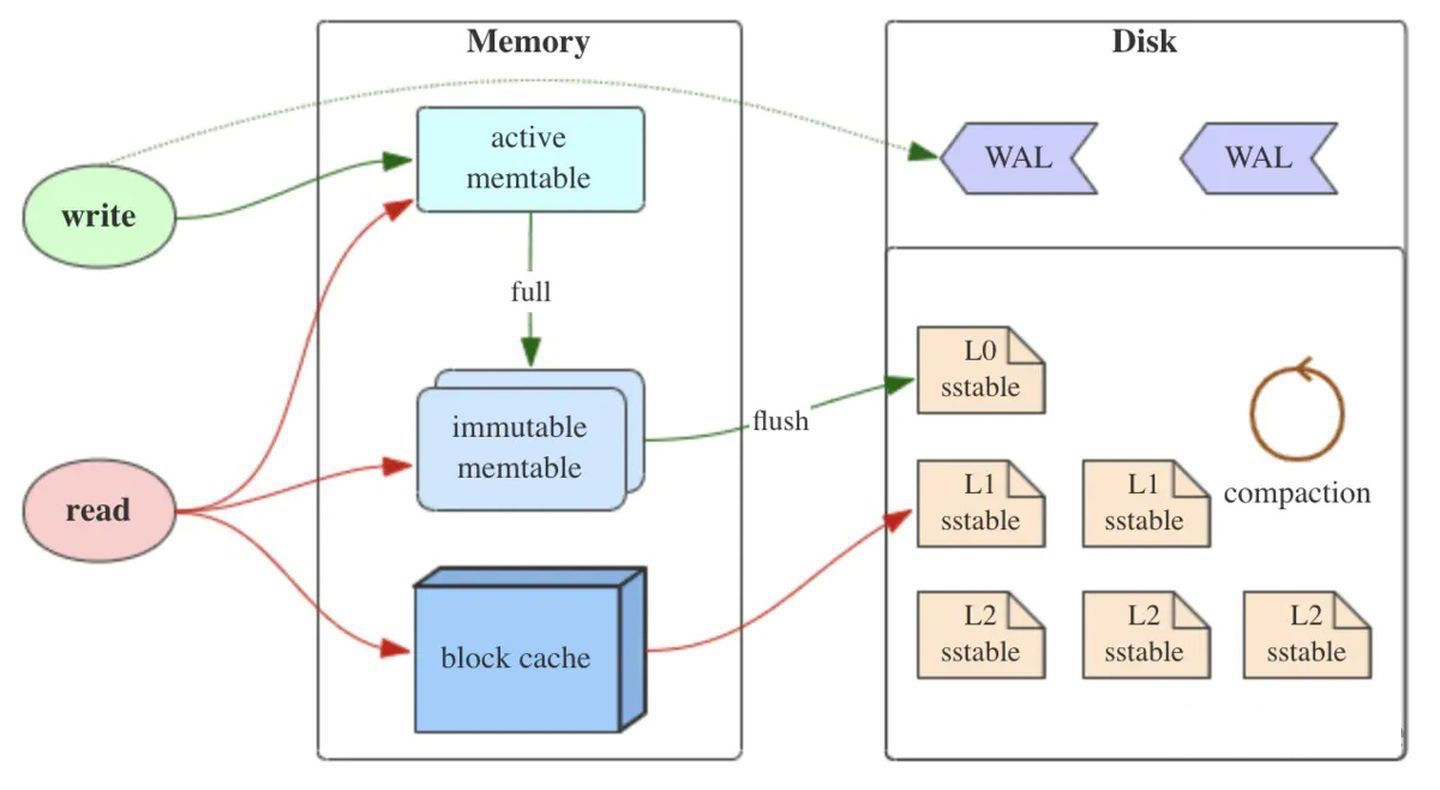
\includegraphics[width=0.8\textwidth]{1.png}
\caption{Component interaction overview}
\end{figure}

\begin{figure}[h!]
\centering
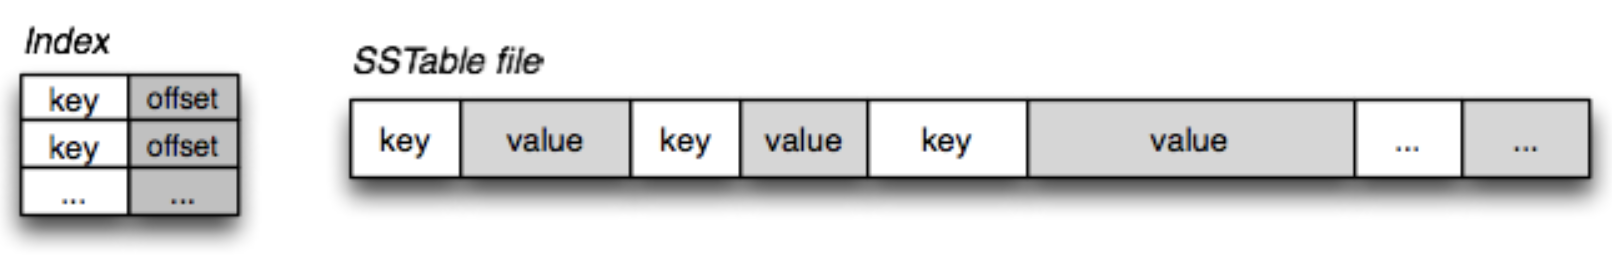
\includegraphics[width=0.8\textwidth]{2.png}
\caption{Parser and AST generation pipeline}
\end{figure}

\clearpage % Force a new page
% Pair 2: Query execution and Storage engine
\begin{figure}[h!]
\centering
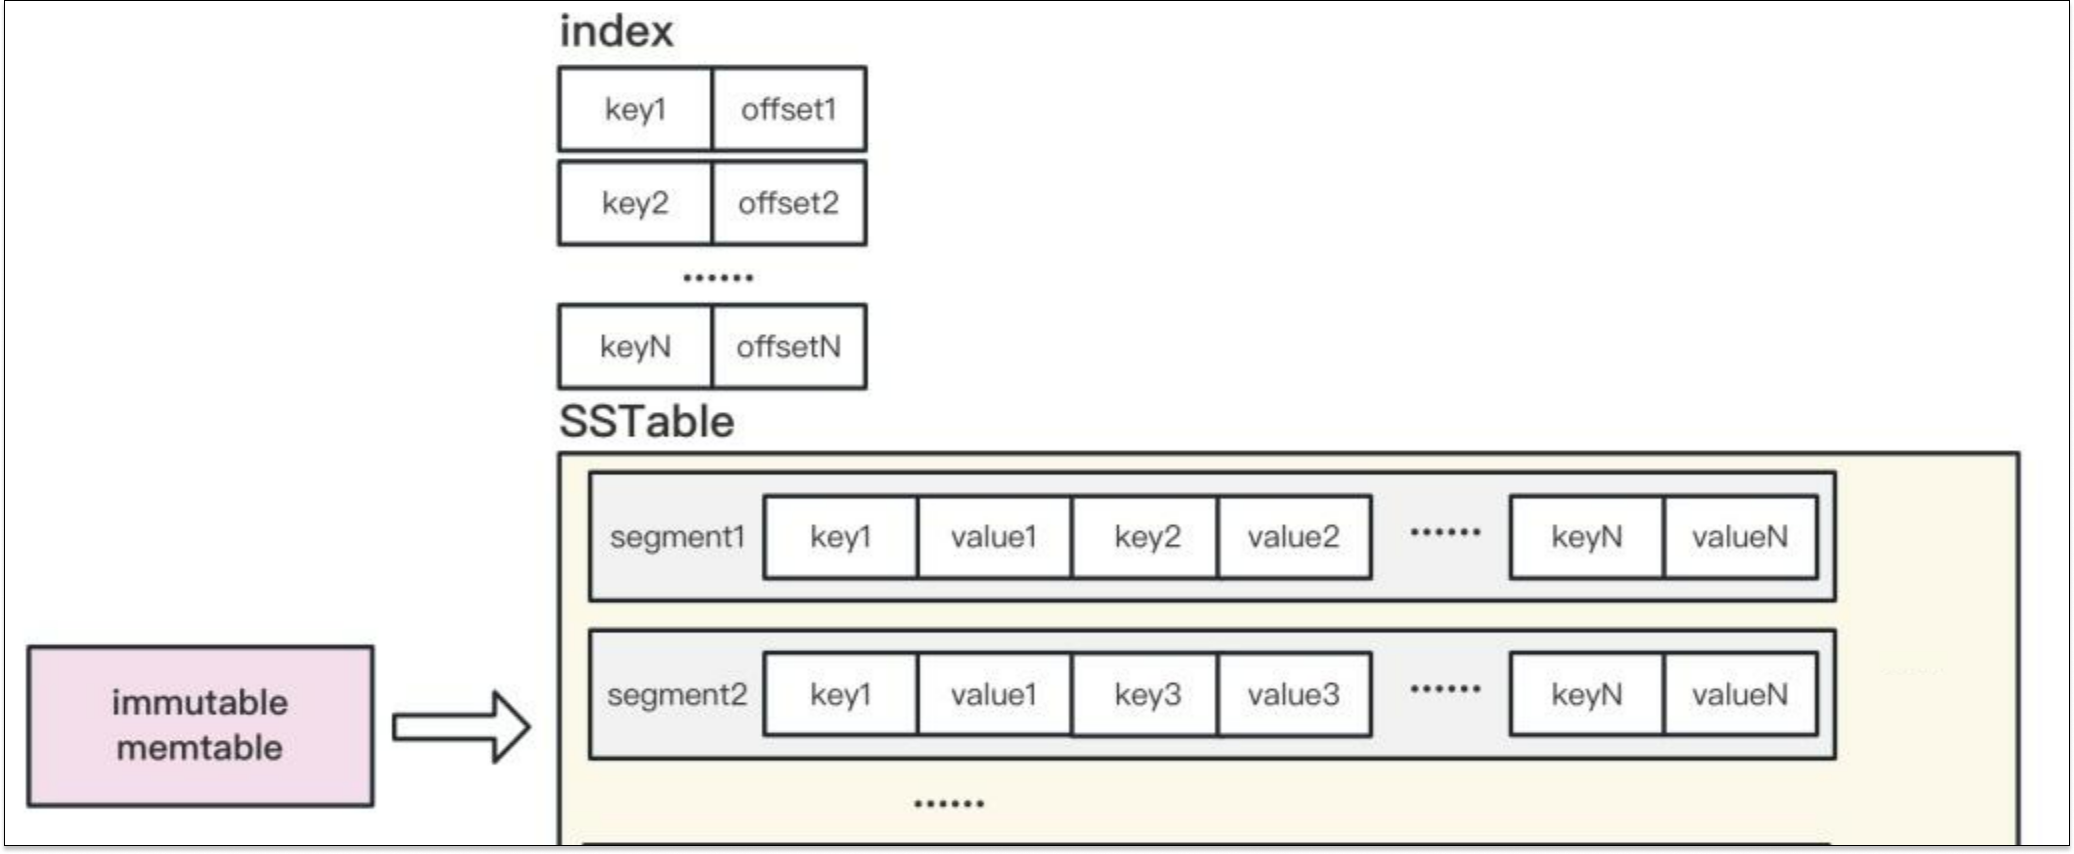
\includegraphics[width=0.8\textwidth]{3.png}
\caption{Query execution workflow}
\end{figure}

\begin{figure}[h!]
\centering
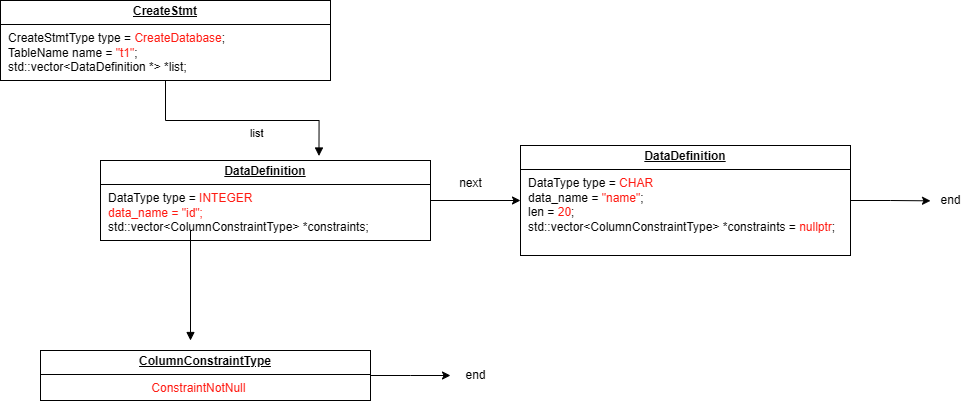
\includegraphics[width=0.8\textwidth]{4.png}
\caption{Storage engine integration}
\end{figure}

\clearpage % Force a new page
% Pair 3: Expression evaluation and Data type
\begin{figure}[h!]
\centering
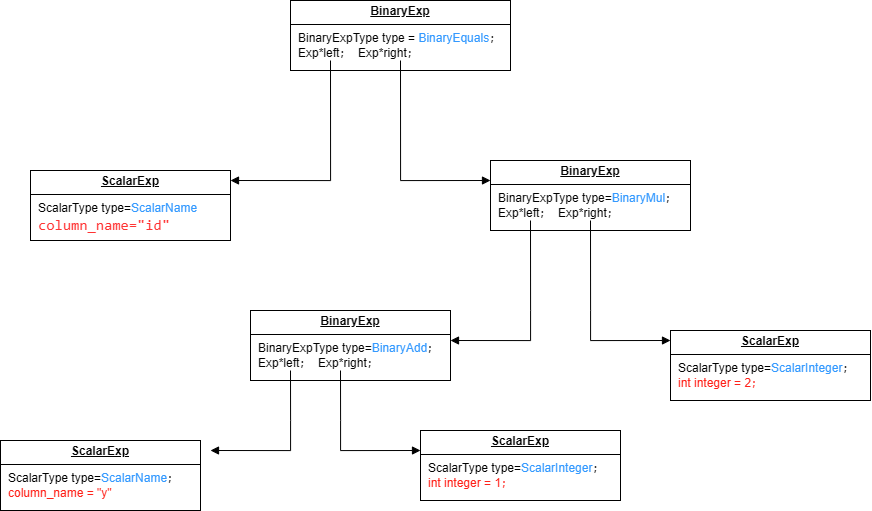
\includegraphics[width=0.8\textwidth]{5.png}
\caption{Expression evaluation system}
\end{figure}

\begin{figure}[h!]
\centering
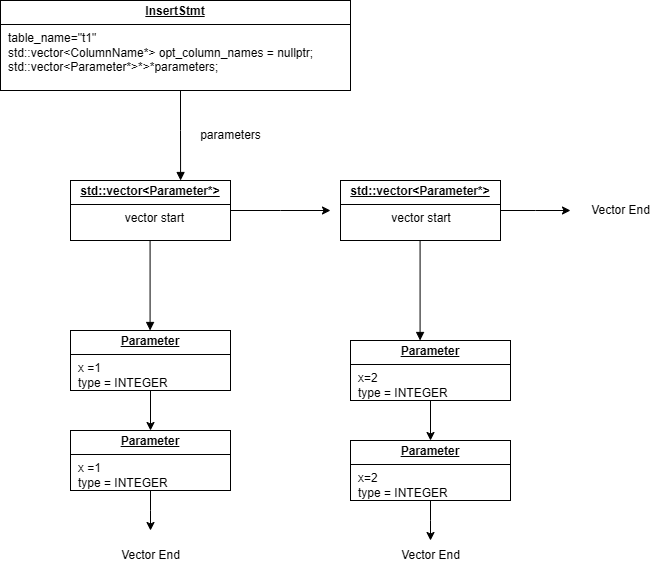
\includegraphics[width=0.8\textwidth]{6.png}
\caption{Data type hierarchy}
\end{figure}

\clearpage % Force a new page
% Pair 4: Constraint enforcement and Transaction management
\begin{figure}[h!]
\centering
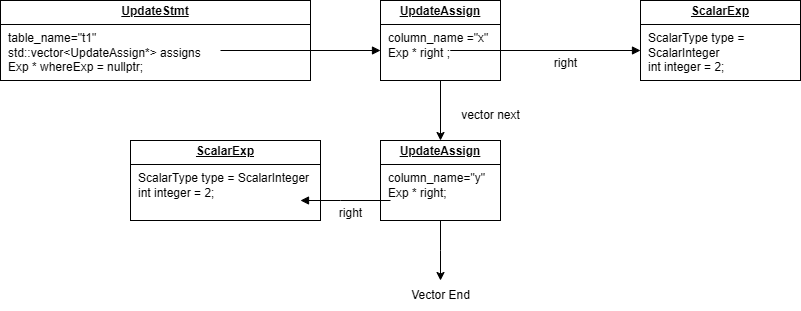
\includegraphics[width=0.8\textwidth]{7.png}
\caption{Constraint enforcement mechanism}
\end{figure}

\begin{figure}[h!]
\centering
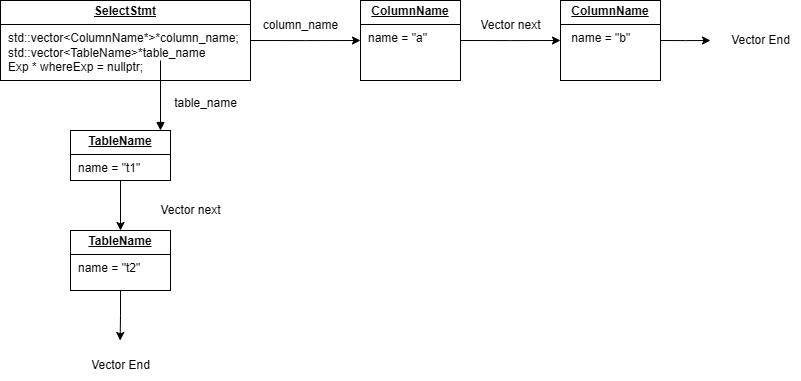
\includegraphics[width=0.8\textwidth]{8.png}
\caption{Transaction management}
\end{figure}

\clearpage % Force a new page
% Pair 5: Error handling and Testing
\begin{figure}[h!]
\centering
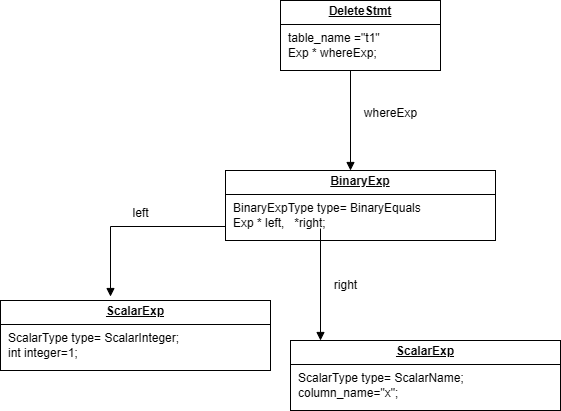
\includegraphics[width=0.8\textwidth]{9.png}
\caption{Error handling subsystem}
\end{figure}

\begin{figure}[h!]
\centering
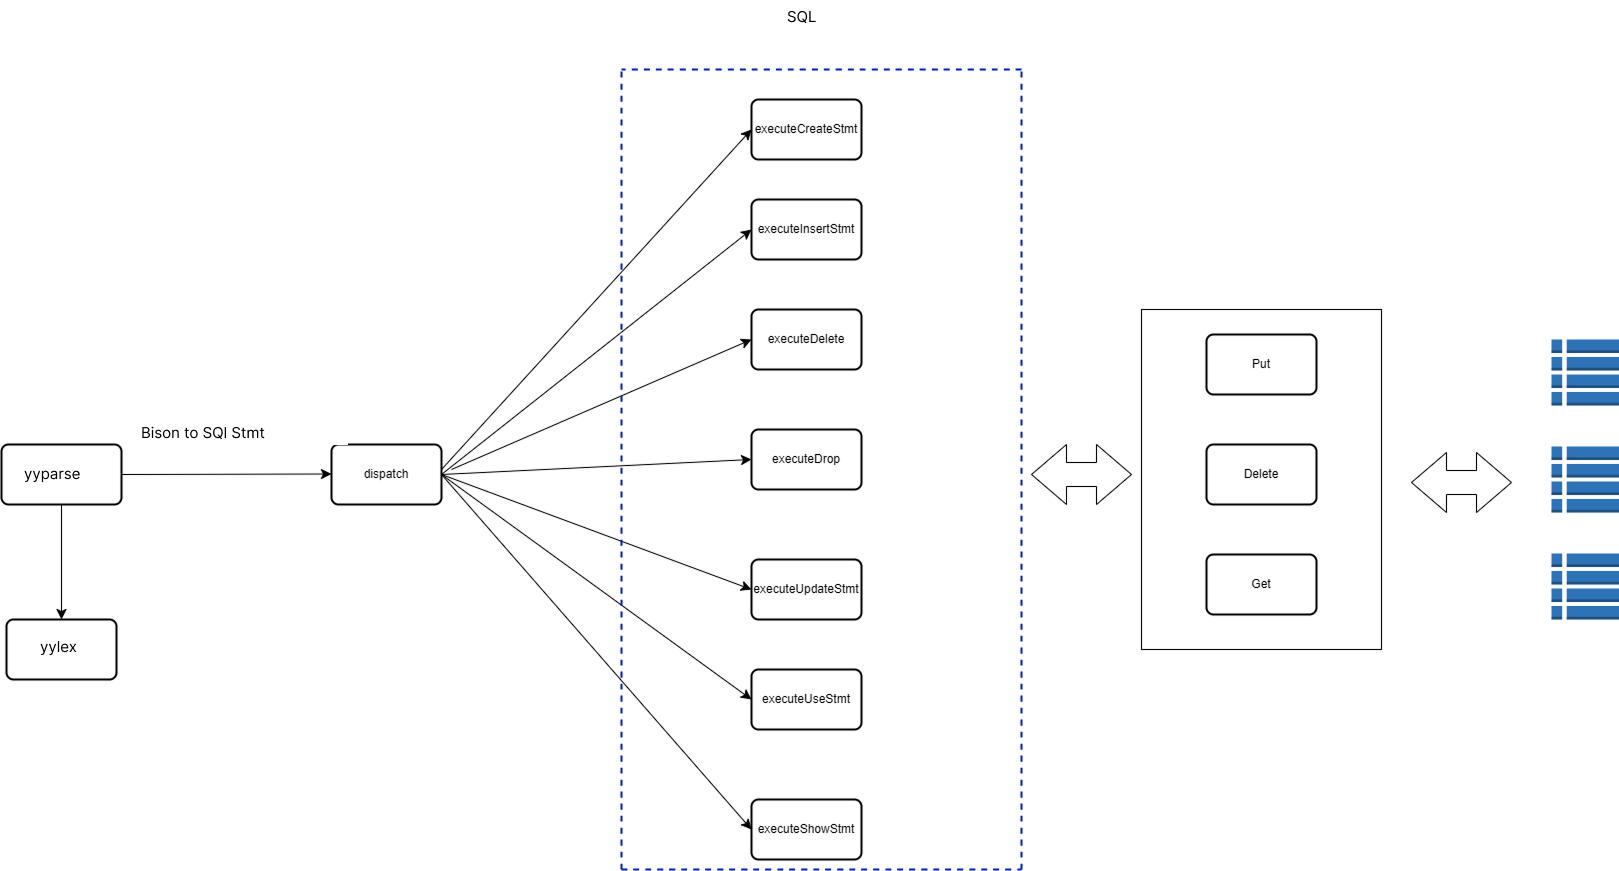
\includegraphics[width=0.8\textwidth]{10.png}
\caption{Testing infrastructure}
\end{figure}

\clearpage % Force a new page to start the next section

\subsection{Key Architectural Components}
The architecture diagrams above illustrate keystoneDB's modular design with clear separation of concerns:

\begin{itemize}
    \item \textbf{Parser Subsystem}: Converts SQL text into a structured AST representation
    \item \textbf{Execution Engine}: Translates parsed statements into operations on the storage layer
    \item \textbf{Storage Manager}: Provides persistence through RocksDB integration
    \item \textbf{Type System}: Enforces data type constraints and conversions
    \item \textbf{Expression Evaluator}: Processes complex query conditions using the visitor pattern
\end{itemize}

This layered approach facilitates maintenance, testing, and extensibility of the system while providing clear educational examples of database internals.

\section{Parser Implementation}
\subsection{Lexical Analysis}
The lexical analyzer (scanner) is implemented using Flex in \texttt{sql.l}. The scanner demonstrates several advanced techniques:

\begin{itemize}
    \item \textbf{Reentrant design}: Uses \texttt{\%option reentrant} for thread safety
    \item \textbf{Case-insensitive token matching}: For SQL keywords
    \item \textbf{Start conditions}: For handling complex tokens like strings and comments
    \item \textbf{Thread-local string buffers}: For safely building string literals
\end{itemize}

\begin{lstlisting}[language=C++,caption=Example of a lexer rule for SQL keywords]
%option reentrant
%%
(?i:SELECT)   { return SELECT; }
(?i:FROM)     { return FROM; }
(?i:WHERE)    { return WHERE; }
\end{lstlisting}

The lexer recognizes the full SQL token spectrum including keywords, operators, identifiers, and literals. It provides detailed error reporting, particularly for unterminated strings and unknown characters.

\subsection{Syntax Analysis}
The syntax analyzer (parser) is implemented using Bison in \texttt{sql.y}. The parser implements a comprehensive SQL grammar with:

\begin{itemize}
    \item \textbf{Type-safe value passing}: Through a \texttt{\%union} structure
    \item \textbf{Precise operator precedence}: Definitions ensuring expressions like \texttt{a + b * c} are parsed correctly
    \item \textbf{Memory management}: Via destructors to prevent leaks from string allocations
    \item \textbf{Error recovery}: Mechanisms for syntax mistakes
\end{itemize}

\begin{lstlisting}[language=C++,caption=Example of union definition and token types]
%union {
    int64_t ival;
    double fval;
    char *str;
    keystoneDB::SQLStmt *stmt;
    keystoneDB::ColumnDef *col_def;
    keystoneDB::TableDef *table_def;
    keystoneDB::DropStmt *drop_stmt;
    keystoneDB::Exp *exp;
    std::vector<keystoneDB::ColumnDef *> *col_list;
    std::vector<keystoneDB::Exp *> *exp_list;
    std::vector<keystoneDB::SelectCol *> *select_list;
    std::vector<keystoneDB::TableRef *> *table_list;
}

%token <str> IDENTIFIER STRING_LITERAL
%token <ival> INTEGER_LITERAL
%token <fval> FLOAT_LITERAL

%token CREATE DROP TABLE DATABASE SELECT
%token INSERT INTO VALUES UPDATE SET
%token DELETE FROM WHERE USE SHOW TABLES DATABASES
%token INT FLOAT CHAR NULL_T NOT IS BETWEEN AND OR
%token EXIT

%left OR
%left AND
%left '=' '<' '>' LE GE NE IS
%left '+' '-'
%left '*' '/' '%'
%left '^'
%right UMINUS
\end{lstlisting}

The parser handles a wide range of SQL statements including DDL operations (CREATE, DROP), DML operations (INSERT, UPDATE, DELETE), and queries (SELECT).

\section{Abstract Syntax Tree Design}
\subsection{Statement Hierarchy}
The project features a sophisticated object-oriented AST design with a hierarchy of SQL statement types:

\begin{figure}[H]
\centering
\begin{tabular}{|c|}
\hline
\textbf{SQLStmt (Base Class)} \\
\hline
\end{tabular}
\newline
\newline
\begin{tabular}{|c|c|c|c|c|c|c|c|}
\hline
CreateStmt & SelectStmt & InsertStmt & UpdateStmt & DeleteStmt & DropStmt & ShowStmt & UseStmt \\
\hline
\end{tabular}
\caption{Inheritance hierarchy of SQL statements}
\end{figure}

All SQL statements derive from a common \texttt{SQLStmt} base class, with specialized implementations for different statement types:

\begin{itemize}
    \item \texttt{CreateStmt} for table and database creation
    \item \texttt{SelectStmt} for data retrieval
    \item \texttt{InsertStmt} for adding records
    \item \texttt{UpdateStmt} for modifying data
    \item \texttt{DeleteStmt} for removing records
    \item \texttt{DropStmt} for schema modifications
    \item \texttt{ShowStmt} and \texttt{UseStmt} for utility operations
\end{itemize}

This hierarchy allows for polymorphic handling of different statement types throughout the execution pipeline.

\subsection{Expression System}
The expression handling system uses an elegant hierarchical design:

\begin{figure}[H]
\centering
\begin{tabular}{|c|}
\hline
\textbf{Exp (Base Class)} \\
\hline
\end{tabular}
\newline
\newline
\begin{tabular}{|c|c|c|c|c|}
\hline
BinaryExp & UnaryExp & ScalarExp & BetweenExp & IsExp \\
\hline
\end{tabular}
\caption{Expression hierarchy in keystoneDB}
\end{figure}

The expression system includes:
\begin{itemize}
    \item \texttt{Exp} base class providing common functionality
    \item Specialized classes for different expression types
    \item Visitor pattern through \texttt{AbstractExpProcessor} to separate expression structure from operations
    \item Support for complex conditions including between expressions and logical operations
\end{itemize}

This design facilitates not just parsing but later stages like optimization and execution as well.

\section{Storage Engine}
\subsection{RocksDB Integration}
keystoneDB uses RocksDB as its persistent storage engine. RocksDB is an LSM-tree-based key-value store that provides high performance for write-heavy workloads.

\begin{lstlisting}[language=C++,caption=Opening a RocksDB database]
rocksdb::DB *db;
rocksdb::Options options;
options.create_if_missing = true;
rocksdb::Status status = rocksdb::DB::Open(options, "/path/to/db", &db);
assert(status.ok());
\end{lstlisting}

\subsection{Data Encoding Strategy}
The project uses a sophisticated encoding approach for mapping relational data to key-value pairs:

\begin{itemize}
    \item \textbf{Table mapping}: Each table receives unique identifiers
    \item \textbf{Primary key encoding}: Records are stored with keys that include table ID and primary key values
    \item \textbf{Secondary index encoding}: Indexes are maintained as separate key-value entries pointing to primary keys
    \item \textbf{Schema storage}: Table definitions and constraints are stored as special system entries
\end{itemize}

This encoding approach is similar to what's used in MyRocks, a MySQL storage engine based on RocksDB.

\subsection{Transaction and Consistency Management}
The system handles transactions and consistency through:

\begin{itemize}
    \item \textbf{Synchronous writes}: For durability-critical operations
    \item \textbf{Snapshots}: For consistent read views during transactions
    \item \textbf{Column families}: For logical separation with atomic write capabilities
\end{itemize}

\begin{lstlisting}[language=C++,caption=Using synchronous writes in RocksDB]
rocksdb::WriteOptions write_options;
write_options.sync = true;
db->Put(write_options, ...);
\end{lstlisting}

\section{Query Execution}
\subsection{Execution Pipeline}
The execution pipeline consists of several stages:

\begin{enumerate}
    \item \textbf{Lexical analysis}: Converting SQL text to tokens
    \item \textbf{Parsing}: Building an AST representation
    \item \textbf{Semantic validation}: Checking against schema information
    \item \textbf{Optimization}: Selecting efficient execution paths
    \item \textbf{Execution}: Translating operations to RocksDB calls
    \item \textbf{Result processing}: Formatting and returning query results
\end{enumerate}

\subsection{Statement Executors}
Each SQL statement type has a corresponding executor:

\begin{itemize}
    \item \texttt{CreateExecutor}: Handles CREATE TABLE and CREATE DATABASE statements
    \item \texttt{SelectExecutor}: Processes SELECT queries with filtering and joins
    \item \texttt{InsertExecutor}: Manages data insertion operations
    \item \texttt{UpdateExecutor}: Handles data modification
    \item \texttt{DeleteExecutor}: Processes data deletion with conditions
    \item \texttt{DropExecutor}: Manages DROP TABLE and DROP DATABASE statements
    \item \texttt{ShowExecutor}: Displays metadata like table list
    \item \texttt{UseExecutor}: Changes the current database context
\end{itemize}

\subsection{Expression Evaluation}
Expression evaluation is handled using the visitor pattern:

\begin{itemize}
    \item \texttt{BinaryEvaluator}: Evaluates binary operations (+, -, *, /, etc.)
    \item \texttt{UnaryEvaluator}: Handles unary operations (-x, NOT x, etc.)
    \item \texttt{ScalarEvaluator}: Processes scalar values (literals, column references)
    \item \texttt{BetweenEvaluator}: Handles BETWEEN expressions
    \item \texttt{ExpChecker}: Validates expressions against schema
\end{itemize}

This approach separates the traversal of expression trees from the operations performed on them.

\section{Type System and Schema Management}
\subsection{Data Types}
keystoneDB supports a set of basic SQL data types:

\begin{itemize}
    \item \texttt{INT}: For integer values
    \item \texttt{FLOAT}: For floating-point numbers
    \item \texttt{CHAR(N)}: For fixed-length character strings
\end{itemize}

\subsection{Constraints}
The system implements basic constraints:

\begin{itemize}
    \item \texttt{NOT NULL}: Ensures a column cannot have NULL values
    \item Primary key support with uniqueness enforcement
\end{itemize}

\begin{lstlisting}[language=SQL,caption=Example of constraint usage]
CREATE TABLE t5 (id INT NOT NULL);
INSERT INTO t5 VALUES (1),(2);
-- The following would cause an error:
-- INSERT INTO t5 VALUES (NULL);
\end{lstlisting}

\subsection{Schema Storage}
Schema information is stored within RocksDB, allowing persistence across database restarts and providing a single source of truth for metadata.

\section{Testing}
\subsection{Unit Testing Framework}
keystoneDB uses GoogleTest for unit testing:

\begin{lstlisting}[language=C++,caption=Example of a unit test for CreateStmt]
// From create_stmt_test.cpp
TEST(CreateStmtTest, CreateTable) {
    // Test setup
    // ...
    
    // Create a table
    auto stmt = new CreateStmt(/*...*/);
    
    // Verify results
    EXPECT_EQ(/*...*/);
}
\end{lstlisting}

\subsection{SQL Test Suite}
The project includes SQL test files:

\begin{lstlisting}[language=SQL,caption=Excerpt from test.sql]
create database test;
use test;
create table t1 (x int,y char(20));
insert into t1 values (42,'hello');
select * from t1;
insert into t1 values (43,'hello');
insert into t1 values (42,NULL);
insert into t1 values (NULL,NULL);
insert into t1 values (99,'hello'),(100,'world');
insert into t1 (x) values (101);
insert into t1 (y) values ('y only');

-- insert test (error expected)
-- Char too long
insert into t1 (x,y) values (101,'looooooooooooooooooooooooooooooooooog');
\end{lstlisting}

These test files cover a range of SQL functionalities including:
\begin{itemize}
    \item Basic DDL operations (CREATE, DROP)
    \item DML operations (INSERT, UPDATE, DELETE)
    \item Queries with filtering (SELECT ... WHERE)
    \item Error handling cases
    \item Expression evaluation
    \item Constraint enforcement
\end{itemize}

\section{Features and Capabilities}
\subsection{Supported SQL Syntax}
keystoneDB supports a substantial subset of SQL:

\begin{lstlisting}[language=SQL,caption=Examples of supported SQL statements]
CREATE DATABASE example;
USE example;
CREATE TABLE user (id INT, score FLOAT);
SHOW TABLES;
INSERT INTO user (id INT NOT NULL) VALUES (1);
SELECT id FROM user WHERE id = 42;
UPDATE user SET id=1 WHERE id=42;
DELETE FROM user WHERE id=42;
SELECT * FROM user WHERE id=(1+2*2+(id=id)+id^id+id) AND id = id%2 AND id IS NOT NULL;
SELECT * FROM t1 WHERE id IS NOT NULL;
DROP TABLE user;
\end{lstlisting}

\subsection{Expression Evaluation}
The system supports complex expressions:

\begin{itemize}
    \item Arithmetic operations: +, -, *, /, \%, \^
    \item Comparison operations: =, <, >, <=, >=, <>
    \item Logical operations: AND, OR
    \item Special conditions: IS NULL, IS NOT NULL, BETWEEN
    \item Nested expressions with proper precedence
\end{itemize}

\begin{lstlisting}[language=SQL,caption=Examples of complex expressions]
SELECT * FROM t2 WHERE ('a'<y AND x>2)=x-1;
SELECT * FROM t6 WHERE id BETWEEN 2 AND 4;
SELECT * FROM t6 WHERE 3 BETWEEN id AND 4;
\end{lstlisting}

\subsection{Multi-Table Operations}
keystoneDB supports joins between tables:

\begin{lstlisting}[language=SQL,caption=Examples of multi-table operations]
-- No ambiguity
SELECT t2.x, t3.x FROM t2, t3;

-- Infer the table that z belongs to
SELECT t2.x, z FROM t2, t4;
\end{lstlisting}

The system handles column ambiguity and qualification appropriately.

\section{Error Handling}
keystoneDB includes comprehensive error handling:

\begin{itemize}
    \item \textbf{Syntax errors}: Detected during parsing
    \item \textbf{Semantic errors}: Like ambiguous column names
    \item \textbf{Constraint violations}: Such as NULL in NOT NULL columns
    \item \textbf{Type mismatches}: For example, string in integer column
\end{itemize}

\begin{lstlisting}[language=SQL,caption=Examples of error cases]
-- Column id can not be NULL
INSERT INTO t5 VALUES (NULL);

-- Char too long
INSERT INTO t1 (x,y) VALUES (101,'looooooooooooooooooooooooooooooooooog');

-- Data type mismatch
INSERT INTO t1 (x,y) VALUES ('100','mismatch');

-- Too many arguments
INSERT INTO t1 (x) VALUES (1,'column mismatch',99);

-- Column count doesn't match value count
INSERT INTO t1 VALUES (1);

-- Unknown column name
INSERT INTO t1 (not_exist_name) VALUES (1,'not exist name');

-- Ambiguous column name
SELECT x, y FROM t2, t3;
\end{lstlisting}

\section{Conclusion}
keystoneDB demonstrates a sophisticated approach to building an educational database management system. The project provides valuable insights into database internals through practical implementation.

The architecture makes thoughtful trade-offs between complexity and capability, with particular attention to:
\begin{itemize}
    \item Memory management
    \item Type safety
    \item Separation of concerns
    \item SQL standard compliance
    \item Error handling
\end{itemize}

This educational DBMS follows the tradition of modern database systems that adapt key-value stores to serve relational workloads, providing a foundation for understanding both traditional relational database concepts and modern storage approaches.

\section{References}
\begin{enumerate}
    \item Key-Value Database, \url{https://en.wikipedia.org/wiki/Key-value_database}
    \item Parsing, \url{https://en.wikipedia.org/wiki/Parsing}
    \item RocksDB, \url{https://github.com/facebook/rocksdb}
    \item SQLite Logic Test, \url{https://sqlite.org/sqllogictest/doc/trunk/about.wiki}
    \item Hyrise SQL Parser, \url{https://github.com/hyrise/sql-parser}
\end{enumerate}

\end{document}
